\section{Hyperscaler}
\textbf{Hyperscaler} sind die führenden Cloud Provider. Die drei Großen sind \textit{AWS}, \textit{Azure} und \textit{Google Cloud}.
\begin{infobox}[Hinweis]
Die Zahlen zu Regionen und Verfügbarkeitszonen sind nur eine Momentaufnahme und ändern sich ständig. Es kommt nicht auf die exakten Werte an, sondern auf die Größenordnung und das Verhältnis der Anbieter zueinander.
\end{infobox}
\begin{table}[H]
    \centering
    \renewcommand{\arraystretch}{1.6} % erhöht den Zeilenabstand
    \begin{tabular}{|p{3.8cm}|p{3.5cm}|p{3.5cm}|p{3.5cm}|}
        \hline
        \textbf{Merkmal}
            & \textbf{Microsoft Azure}
            & \textbf{Amazon Web Services}
            & \textbf{Google Cloud Platform} \\
        \hline
        \textbf{Regionen}
            & 33 Regionen
            & 49 Regionen
            & 40+ Regionen \\
        \hline
        \textbf{Verfügbarkeitszonen}
            & 105 Zonen
            & 148 Zonen
            & 121 Zonen \\
        \hline
        \textbf{Besondere Datendienste}
            & Azure Synapse Analytics, Azure Cosmos DB
            & Amazon Redshift, DynamoDB
            & BigQuery (serverloser Data Warehouse Dienst), Spanner \\
        \hline
        \textbf{Typische Anwendungsfälle}
            & Unternehmen mit Microsoft-Umgebung, Hybrid Cloud, Legacy-Migration
            & Startups, große skalierbare Workloads, breite Service-Auswahl
            & ML-lastige Anwendungen, Big Data, Cloud-Native-Entwicklung \\
        \hline
        \textbf{Marktposition}
            & Nr. 2 weltweit
            & Nr. 1 weltweit
            & Nr. 3 weltweit \\
        \hline
    \end{tabular}
    \caption{Vergleich der Cloud-Anbieter: Azure, AWS und Google Cloud Platform}
    \label{tab:cloud-anbieter-vergleich}
\end{table}


\begin{figure}[H]
    \centering
    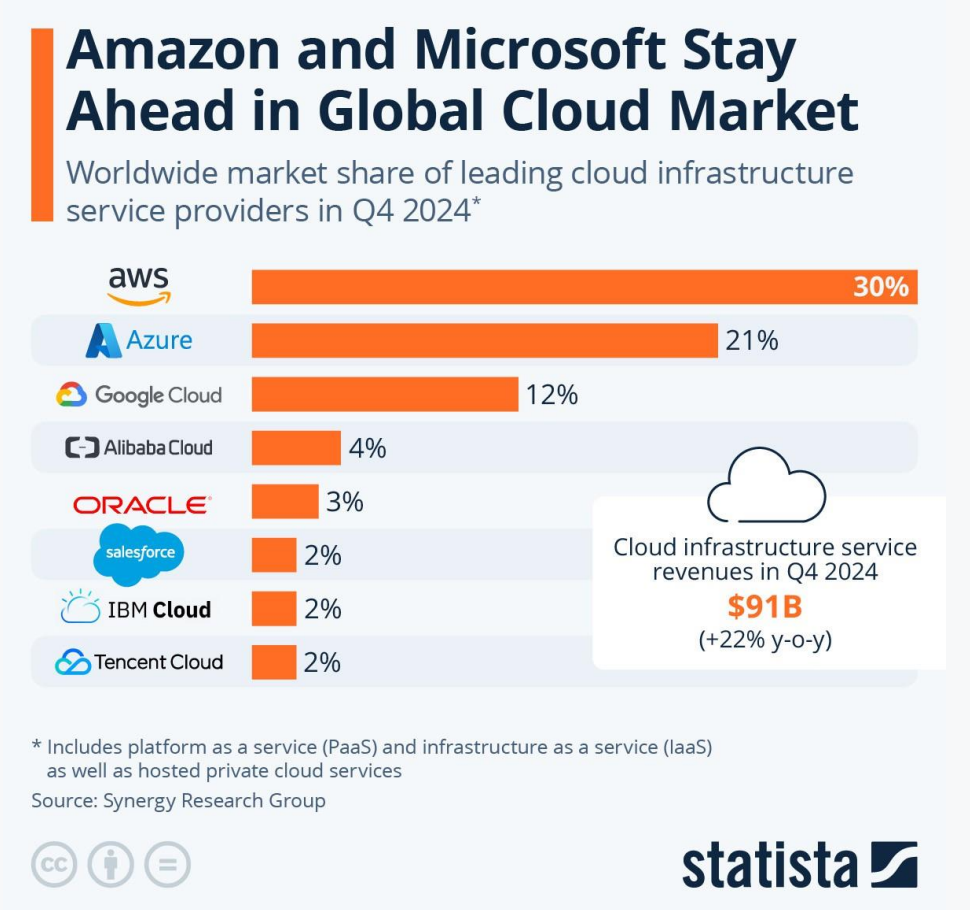
\includegraphics[width=\textwidth]{assets/images/HyperscalerMarketshare}
    \caption{Marktanteil der Cloudprovider.}
\end{figure}